---
title: Clean code
author: Dimitri Merejkowsky
---

#

\huge \center What is Clean Code?

# Well, let's clean some code!

\large \center Example with fizzbuzz

# A quote

> "Any fool can write code that
> a computer can understand.
> Good programmers write code
> that humans can understand."

Martin Fowler

# Code quality

*Hugely subjective*

But matters a lot!

# Measuring code quality

You need to ask the team!

# An illustration

![](./wtf.png)

# An other definition

> “Clean code always looks like it was written
> by someone who cares

Michael Feathers

# Sad fact

The natural tendency of any code base is for the code quality to *degrade*.

Maintaining code quality is always a challenge.

(Known as "the flappy bird problem)

#

\huge \center Advice

# Take your time!

It's usually better to have 80\% well done than 100\% with lower quality
and more rush.

*Note: some teams don't apply this - but usually they're not crafters
either*

# Boy scout rule

Try and leave the code a little better than you found it.


# The psychopath


\includegraphics[width=7cm]{shining.png}

> “Always code as if the person who ends up maintaining your code
> will be a violent psychopath who knows where you live.”

Martin Golding

Usually, the violent psychopath is you!

# Broken Window

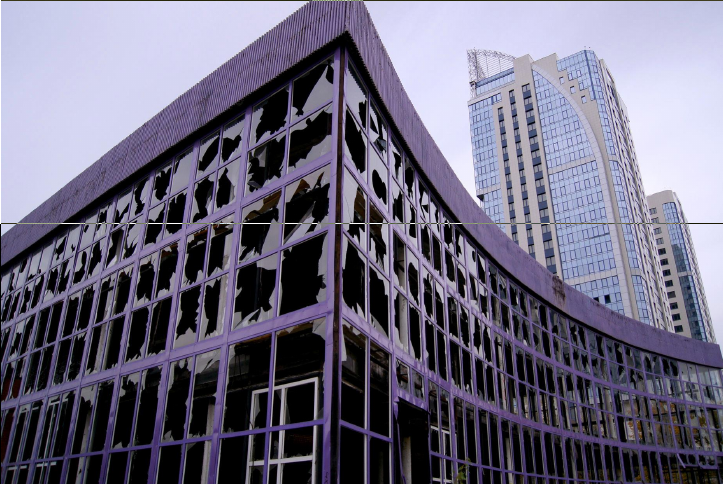
\includegraphics[width=7cm]{broken-windows.png}

# Avoid metrics

Metrics can be gamed.

Just because it's easy to measure, does not mean it's relevant.

#

\huge \center What the science has to say


# sleep is important

Don't work late ! And make sure to sleep well.

\vfill

You'll write really bad code when you're sleep deprived, and you'll be
*unable to notice how bad you are working*.

# Code review works

Go ask other people to read and comment your code. It's what I do when I
grade you, and it's how open source works

# Tests matter

In fact, it's a topic in itself - spoiler for later :)

#

... and that's all. The *science* of software development has yet to reach
consensus on *anything* but the importance of good sleep and code reviews.

And there's debate to know if there are more efficient things than code
reviews, by the way.


#

\huge \center Clean code basics

# Conventions

Follow established Conventions.

Python has PEP8:  https://www.python.org/dev/peps/pep-0008/

... and write code in English.

(Unless the core domain is in French)

#

\huge \center Comments

# Comment position

Either:

* on an other line, before the described code
* on the same line, after the described code

\vfill

```python
# example 1 - a long comment talking
# about foo() and bar() ...
foo()
bar()

x = spam  # short comment on x
```


# Comments (1)

Do not put useless comments:

```python
# foo.py written by John Doe. Last modified on 2021-03-31
```

* We already know the file name because  we've just opened it!
* We often know (or don't care) about the author name
* Ditto for date of last change (which you'll forget to update)

\vfill

This is sometimes called *rotten* comments.

# Comments (2)

Do not put useless comments (2)

```python
# Adds to to x
# x : the number to add 2 to.
# Returns the result of adding 2 to x
def add_two(x):
    return x + 2
```

\vfill

We can know all this by looking at the code!

# Comments (3)

Do not leave dead code:

```python
def do_stuff():
    # x = do_x_v1()
    # y = do_y_v2()
    # z = combine(x, y)
    x = do_x_v2()
    y = do_y_v2()
    z = combine_v2(x, y)
```

Dead code also *rots* and *smells*.


# Comments (3)

Do insert comments when the code is not enough.

Try to describe *why*, not *how*.

Further reading:

https://hackaday.com/2019/03/05/good-code-documents-itself-and-other-hilarious-jokes-you-shouldnt-tell-yourself/

# Docstrings

Other type of comment:

```python
def do_stuff():
    """ A string below the function

    """
    ...
```

# Docstrings - when to use them

Lots of debate.

What I do:

* Put them in *all* public methods if you are writing a library

* Use them as high-level descriptions of tests

```python
def test_complex_feature():
    """ Scenario:
    Given ..
    When ...
    Then ...
    """
    # lots of code here
```

#

\huge \center Naming

\vfill

\normalsize One of the hardest problems in computer science

# Some rules

* Be consistent
* Don't use abbreviations
* Don't put the type in the name
* Use a descriptive name

\vfill

```python
age = 16  # too short
minimal_age = 16 # nice
minimal_age_to_be_able_to_drive  16  # to long
```

# Plural and singular

Use plural if it's a collection.

```python
for foo in foos:
    ...
```

Or sometimes there's a nicer word:
```python
for animal in zoo:
    ...
```

```python
# An example from Bouygues
for ligne in parc:
  ...
```

# Use good metaphors

Use names you could explain to the rest of the team.

\vfill

*Bad*: "Unlock Device"

*Good*: "Verify Identity"

# Rules for variable name size

Big scope, long name

Short scope, small name.

In Python, you are allowed one-letter variables names in `for` loops
and list comprehensions but almost nowhere else.

#

\huge \center Functions


# Grammar for function names

Use verbs at the imperative, present tense

```python
# Good
def display_tree():
    ...

# Bad
def displays_the_tree():
    ...

# Bad
def tree_display():
    ...

```

# Generic vs specific functions

The more generic the function, the shorter the name

```python
def make_coffee(*, sugar=True):
    if sugar:
        make_coffee_with_sugar()
   else:
        make_coffee_without_sugar()
```



# Returning booleans

Use `is_`, or `has_`, etc so that the code reads better:

```python
if is_allowed_to_drive(person):
    ...
```

# How big should my function be?

Functions should be really short.

# Code smell (1)

A function that looks like this ...

```python
def my_big_function():
    # step 1
    ...

    # step 2
    ...

    # step3
    ...
```

... can probably be split in 3 (the comments are the clue)

## Code smell (2)  Number of arguments

* 0 to 3 : probably fine
* more than 3 : danger -> consider introducing
  a class for the parameters

\huge \center Clean code and Craft

# Digression - dev cycle

# Cycle en V

![](./cycle-en-v.png)

This one does not really work ...

# More realistic dev cycle

![](./cycle-dev.png)

\vfill

You always use this one (even if you don't know it)

# Catching problems early matter

The later you are in the dev cycle, the harder
it becomes to fix the bug

So you want *short* feedback loops.

# Craft

* Nous sommes des artisans
* Nous entretenons le code comme si c'était un jardin
* Nous utilisons des bonnes pratiques et nous les transmettons

# Bonnes partiques clean code

* Le refactoring
* Les tests

Comment garantir la qualité du code, le fait qu'il soit testé *et* la qualité des tests?

# TDD

A cycle

* Red -> 1 failing test
* Green -> all tests pass
* Refactor -> stop - refactor both production and test code



# TDD - why it works

* Red: clarifying intents and specifications
* Green: implementing the feature
* Refactor: you know tests will catch most of the mistakes

## TDD - 3 phases

* Red: focus on specs
* Green: focus on implementation, algorithms, data structures and so on
* Refactor: focus on quality

## TDD - Short cycles

 * Get feedback fast
 * Find bugs early
 * Also get feeback on the architecture while you're building it


#

\huge \center Clean code and Classes

# Naming

Classes names are *nouns* and start with an uppercase letter.

Avoid meaningless words like `Handler`, `Manager`, `Data`, `Info` ...

# Foreword

Classes, composition and inheritance are powerful but *dangerous* tools.

* They hide the control flow.
* It's very easy to make a mess!

# Avoid inheritance

Lots of powerful and dangerous features:

* Multiple inheritance (for languages that have them)
* Some attribute may be shared

#  My advice

* Only every inherit from *one* parent
* Use inheritance for exceptions
* Use inheritance for abstract base classes (more on this later)

\vfill

And that's all!

#

\huge \center Packages and modules

# Naming

Use short names, in `lower_case`


# Avoid stutter

```python
# in fractions.py
class Fraction:
    ...
```

```python
# Bad:
def add_fraction(fraction_a, fraction_b):
    ...
```

```python
# Better
def add(a, b):
    ...
```

# For the caller

```python
# We know we're adding functions
from fractions import add
res = add(f1, f2)
```

\vfill

Worried about collisions?

```python
import fractions
import vectors

f3 = fractions.add(f1, f2)
v3 = vectors.add(v1, v2)
```

#

\huge \center Clean architecture

# What is architecture?

Basically, the collection of modules, classes and methods that will
be used throughout the project.

This is more high-level than the *contents* of the classes, modules, and functions.


# Rules of architecture

The _rules_ of architecture do not depend on the language.

Software is made of:

* sequence
* selection
* iteration

(It never changed for the last 50 years)

So if the nature of the code did not change, the rules of architecture did
not change either.

#

Architecture, design, and programming are the same thing - the only difference
is how high-level they are.

Corollary: architects who do not write code, or programmers who do not think about
high-level design are not doing their best.

#

\huge \center APIs


# Definition

Application Programming Interface

A set of functions (or methods) or class you can use
as an *external* user of a piece of code

# APIs and libraries

Often you use an API from a library.

Example with `datetime`:

https://docs.python.org/3/library/datetime.html

# What makes good APIs

* Good naming
* Good metaphors
* Consistency
* Easy to use
* Hard to misuse
* Simple things should be easy, complex things should be possible

# Making good APIs

It's *hard*

What can help:

* Brainstorms
* Tests
* Documentation
* Examples
* Review

And you should do all  of this *before* writing the production code, because
architecture is much harder to change afterwards!

# The big problem with APIs

They are hard to change.

Sometimes they *break*, which means *all the code that use them* must change,
and that can have really bad consequences.

# The bad news

As soon as you *write a function* in a piece of code, you *are* defining
an API from the point of view of the rest of the code.

All of the above applies (minus the fact breaking them is not as bad)

# My advice

Treat any piece of code as it was part of a public library usable by anyone.

#

\huge \center Object Oriented Programming

# Object Oriented Programming

One definition: put *data* and *behavior* that operate on this data in
the same place.


Note: not necessarily achieved with classes. It's mostly a way
of *structuring* code


# Encapsulation

The big idea: users of a class should not *need to know* about
how it works internally.

# Example: the counter class

```python
class Counter:
    def __init__(self):
        self._tally = 0

    def add(self, count):
        self._tally += count

    def get_total(self):
        return self._tally
```

* `Counter(), add(), total()`: public interface
* `_tally`: private implementation detail

# An other example

```python
class Person:
    def __init__(self, first_name, last_name):
        self.first_name = first_name
        self.last_name = last_name

    @property
    def full_name(self):
        return f"{self.first_name} {self.last_name}"
```

* `first_name` and `last_name` are read/write
* `full_name` is read-only

# Example

```python
p = Person("John", "Smith")  # OK
p.last_name = "Smith-Brown"  # OK
print(p.full_name)           # OK
p.full_name = "John Brown"   # Error
```

# Invariant

We say the class enforces an *invariant*

The full name will *always* be the concatenation of `first_name`
and `last_name`.

The tally will *always* contain the running total of calls to `add`.

# Basic principles

1. Passes all the tests
1. Minimize duplication
1. Maximize clarity
1. Fewer elements

# How to get clean architecture

* Make it work, make it right, make it fast
* Use TDD!
* Always look back at the architecture

# More advanced principles

* Sing Level of Abstraction
* Law of Demeter
* Tell, don't ask - Command/Query Separation
* Calisthenic objects
* SOLID
* DDD tactics

...

And more

# Advice for principles

* They are abstract
* They often contradict each other

\vfill

Don't try and follow all of them at once!


# Law of Demeter

Formulation:

You should *not* access the *fields of the field* of an other class

# Example

```python
class User:
    def __init__(self, name, department=None):
        self.name = name
        self.department = department

def get_user_info(user)
    user_name = user.name  # OK
    if user.department:
        department_name = user.department.name  # Bad!
    else:
        department_name = None

    if department_name:
        return f"{user_name} from {department_name}"
    else:
        return user_name
```

# Why?

We have a coupling between get_user_info() and user (which is fine)

\vfill

But the `get_user_info()` method *knows* that:

* users belong to 0 or 1 department
* every department has a name

(which is tighter coupling and *not* fine)


# When the specifications change

Let's say users can belong to *one or more* departments.

Now we need to change `get_user_info`, which a sign of *fragility*.

# When the specifications change (2)

```diff
def get_user_info(user)
    user_name = user.name
-    if user.department:
-       department_name = user.department.name
+    if user.departments:
+       first_department = user.departments[0]
+       department_name = first_department.name
    else:
        department_name = None

    ...
```


# The fix

Move the coupling from `get_user_info` and `Department` inside `User`

```python
class User:
    def get_department_name(self):
        department = self.department
        if department:
            return department.name

def get_user_info(user):
    user_name = user.name
    department_name = user.get_department_name()
    return f"{name} from {department}"
```

# Before

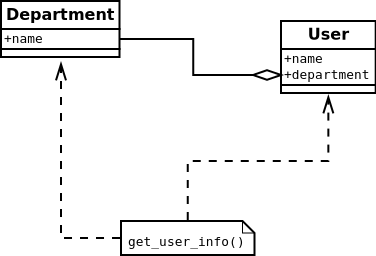
\includegraphics[width=8cm]{demeter-1.png}

# After

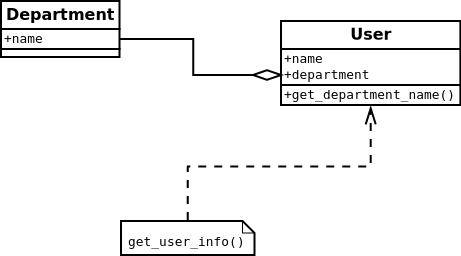
\includegraphics[width=8cm]{demeter-2.png}

# When the specifications change (after)


```diff
class User:
- def __init__(self, name, department=None):
+ def __init__(self, name, departments=None):
        self.name = name
-        self.department = department
+        self.departments = departments
```

```diff
class User:
   def get_department_name(self):
-       if self.department:
-           return self.department.name
+       if self.departments:
+           first_department = self.departments[0]
+           return first_department.name
+
```

`get_user_info()` did not need to change!

# Command/Query separation

* Command: change state

* Query : return some state

# Command/Query separation

Either:

Command: returns nothing, has side effects

Query : returns something, has no side effects

\vfill

Avoid side-effects in a function that returns a value!

# SRP

Single responsibility principle

A class/module should have only *one* reason to change.

* What are the things that can change?
* Who might be asking for these changes?

# SRP

Smells:

* A place where code keeps changing
* Conflicts happening in the same file
* Rigid code

#

\huge \center Going further

#

* SOLID
* CUPID: https://dannorth.net/2022/02/10/cupid-for-joyful-coding/
* Many, Much, More, Smaller Steps: https://www.geepawhill.org/series/many-much-more-smaller-steps/
* Primitive Obsession
* Behavior Drive Development
* Domain Driven Design
# Tools for clean code

## On tools

Use the same tools as your team, or be ready to face
problems you're the only one having :)

## IDEs

IDEs can help

* Code navigation
* Code completion (useful for long_names ;)
* Refactoring tools
* ... and more

## Linters

Code that will read your code and tell you about problems

For instance:

```python
if is_full_moon():
    mesage = "Attention aux loug-garous"
else:
    message = "Promenons-nous dans les bois"
print(message)
```

## Linter (2)

```
moon.py:7:9: F841 local variable 'mesage' is assigned to but never used
```

Should have waiting for a full moon to see the bug otherwise!

## Formatter

Demo!

## Formatters

* The less configuration the better
* black for Python, gofmt for Golang
* Use IDE for C# Java
...

## Code manifesto

You'll often have debates about clean code during code review

My advice : take a decision and write it into a "code manifesto"

The actual *contents* does not matter much

# Example (1)

I use do write:

```
x = list()
y = dict()
```

Now I write

```
x = []
y= {}
```

# Example

Both are *fine*, actually. What matter is to not mix the two!

Beware of 'post-hoc' arguments ;)

Debates is usually not productive, so try to limit its impact
on productivity
